\chapter{Аналитический раздел}
\label{cha:analysis}
В данном разделе анализируется предметная область и определяются требования к разрабатываемой системе.

\section{Анализ предметной области}
Процесс подбора персонала проходит в несколько этапов. Первый этап производится в отраслевой организации. При этом учитываются такие критерии, как график работы, отношение к командировкам, минимальная и максимальная заработная плата, знание языков, образование, желаемая должность и опыт работы в аналогичной сфере. Последний этап заключается в собеседовании кандидатов менеджерами компании.

Распределенная система включает в себя взаимодействующие между собой организации, такие как компании-наниматели, кадровое агентство(и оно же - база резюме), отраслевые организации.

Каждая из систем представляет собой независимый субъект, обладающий своей логикой и базой данных. Субъекты взаимодействуют между собой по публичным каналам передачи данных (как синхронным, так и асинхронным).

Схема предметной области представлена на рисунке ~\ref{fig:idef0} в виде диаграммы IDEF0.

\begin{figure}[ht]
\centering
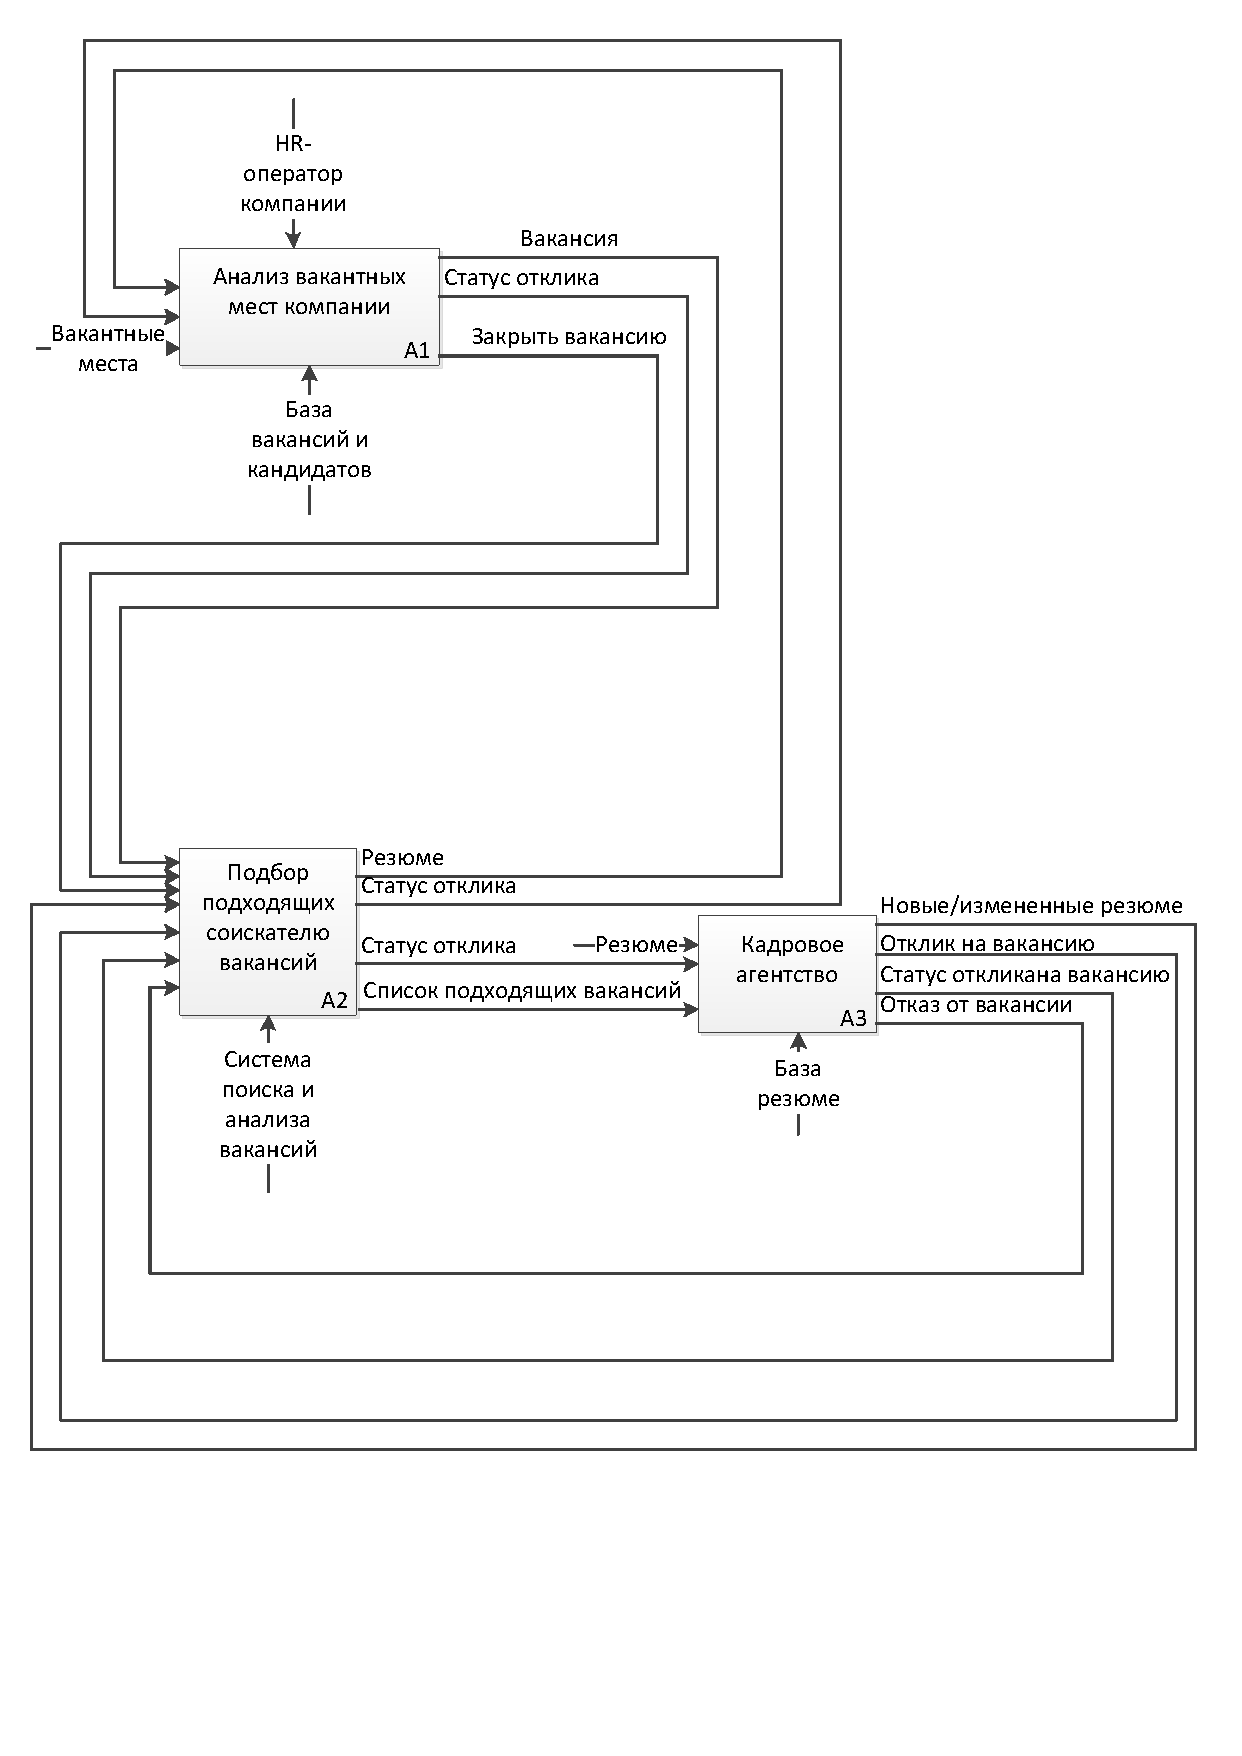
\includegraphics[width=\textwidth]{include/idef0.pdf}
\caption{Схема предметной области}
\label{fig:idef0}
\end{figure}

\section{Описание системы}
Разрабатываемая РСОИ состоит из трех типов узлов:
\begin{enumerate}
\item кадрового агентства;
\item отраслевой организации;
\item компании-нанимателя;
\end{enumerate} 

Рассмотрим функционирование каждого узла.
\begin{enumerate}[1.]
\item Кадровое агентство предоставляет соискателям графический интерфейс для создания резюме и обеспечивает удобное взаимодействие с предлагаемыми вакансиями от компаний-нанимателей.
\item Отраслевая организация принимает заявки от узлов компаний-нанимателей и кадровых агентств и обеспечивает логику обработки поступающих данных. А главное, на нем автоматически для каждой поступившей вакансии запускается поиск подходящих кандидатов, а для каждого нового кандидата список возможных вакансий.
\item Узел компании-нанимателя предоставляет интерфейс для оператора HR-отдела, позволяющий создавать заявки о вакантных местах с указанием критериев к соискателям, а также отклонять или принимать отклики от возможных кандидатов.
\end{enumerate}

\section{Сценарии функционирования системы со стороны соискателя}
\subsubsection{Регистрация соискателя}
Регистрация позволяет завести резюме.
Для регистрации надо:
\begin{enumerate}
\item указать имя, фамилию, отчество и дату рождения (зарегистрироваться может только совершеннолетний соискатель)
\item указать адрес электронной почты. Надо указывать реальный адрес, по которому в дальнейшем с вами свяжутся работодатели.
\item указать пароль
\end{enumerate}
\subsection{Аутентификация соискателя}
Аутентификация возможна только для зарегистрированных пользователей. Аутентификация позволяет просматривать и редактировать данные о себе, а также взаимодействовать с предлагаемыми вакансиями.
Для аутентификации надо:
\begin{enumerate}
\item указать адрес электронной почты в качестве логина
\item указать пароль
\end{enumerate}
\subsection{Заполнение данных об образовании}
Данные о вузе и специальности служат одним из критериев отбора, поэтому важно заполнить информацию об уже полученном (или получаемым в данный момент) образовании. Также немаловажную роль играет знание соискателем языков.
Заполнение данных о себе:
\begin{enumerate}
\item пройдите процедуру аутентификации соискателя
\item чтобы приступить к заполнению данных, выберите вкладку "Редактировать данные о себе" 
\item для того чтобы добавить образование, нажмите на кнопку "Добавить университет"
\item выберите название университета
\item выберите тип обучения
\item напишите свою специальность
\item укажите дату окончания университета
\item для того чтобы удалить данные об этом образовании, нажмите "Удалить университет"
\item для того чтобы добавить данные о знании языка, нажмите кнопку "Добавить язык"
\item выберите язык из списка
\item выберите уровень владения языком
\item чтобы данные были сохранены в базе, нажмите кнопку "Сохранить"
\end{enumerate}
\subsection{Создание резюме/поиск работы}
Только после создания резюме, данные соискателя будут отправлены на узел отраслевой организации. В резюме указываются не только возможности кандидата, но и его пожелания к будущей должности. От выбора сферы деятельности, зависит то, в какую отраслевую организацию будет отправлено резюме.
Чтобы создать/изменить резюме:
\begin{enumerate}
\item пройдите процедуру аутентификации соискателя
\item чтобы приступить к заполнению данных, выберите вкладку "Резюме" 
\item для добавления нового резюме, нажмите кнопку "Добавить резюме"
\item выберите интересующую отрасль из списка
\item выберите график работы
\item выберите график командировок
\item введите максимальную и минимальную заработную плату, которую вы ожидаете
\item введите желаемую должность
\item заполните данные о работе в аналогичной сфере - навыки, опыт работы (в годах)
\item Для внесения изменений в базу, а также отправку данных отраслевым агентствам, нажмите "Сохранить/Обновить резюме" 
\end{enumerate}
\subsection{Отказ от рассмотрения вакансии на любом этапе оценки кандидата}
Соискатель имеет полное право отказаться от вакансии, если она для него больше не актуальна, также он может отказаться даже от просмотра ее в списке возможных предложений, в таком случае, компания еще не знает о наличие кандидата и соотвественно, ей не отсылается сообщение с отказом.
\begin{enumerate}
\item пройдите процедуру аутентификации соискателя
\item если нет резюме или оно уже устарело, создайте/измените его на вкладке "Резюме"
\item выберите вкладку "Показать вакансии"
\item нажмите кнопку "Отказать" под выбранным предложением вакансии. 
\end{enumerate}
\subsection{Переход кандидата к очередному этапу отбора}
\begin{enumerate}
\item пройдите процедуру аутентификации соискателя
\item если нет резюме или оно уже устарело, создайте/измените его на вкладке "Резюме"
\item выберите вкладку "Показать вакансии"
\item нажмите кнопку "Принять" под выбранным предложением вакансии
\end{enumerate}

\section{Сценарии функционирования системы со стороны оператора HR-отдела компании}
\subsection{Создание вакансии/поиск кандидатов}
\begin{enumerate}
\item выберите вкладку "Редактор вакансий"
\item введите название позиции
\item введите требования к кандидату в поле "О позиции"
\item выберите отрасль
\item выберите график работы
\item выберите график командировок
\item введите минимальную и максимальную зарплату, на которую может рассчитывать кандидат
\item введите ожидаемый минимальный опыт работы кандидата
\item для добавления требований к знаниям языков, нажмите кнопку "Добавить языковые требования к кандидату" и выберите язык и уровень владения языка
\item для удаления требований к знаниям языков, нажмите кнопку "Удалить язык"
\item для добавления требований к образованию кандидата, нажмите кнопку "Добавить ожидаемое от кандидата образование", выберите университет и введите специальность
\item для удаления требований к образованию кандидата, нажмите кнопку "Удалить образование"
\item чтобы сохранить введенные данные в базе и отправить данных отраслевым агентствам, нажмите "Сохранить позицию" 
\end{enumerate}
\subsection{Отказ от рассмотрения кандидата}
\begin{enumerate}
\item если нет сохраненных вакансий или они устарели, создайте или измените позицию
\item выберите вкладку "Возможные кандидаты"
\item выберите соответствующего кандидата
\item нажмите кнопку "Отказать"
\end{enumerate}
\subsection{Переход кандидата к очередному этапу отбора}
\begin{enumerate}
\item если нет сохраненных вакансий или они устарели, создайте или измените позицию
\item выберите вкладку "Возможные кандидаты"
\item выберите соответствующего кандидата
\item нажмите кнопку "Принять"
\end{enumerate}
\subsection{Закрытие вакансии}
\begin{enumerate}
\item выберите вкладку "Редактор вакансий"
\item для удаления вакансии, нажмите "Удалить позицию"
\end{enumerate}

Основной сценарий взаимодействия пользователя с системой представляет собой последовательность следующих действий:
\begin{enumerate}
\item пользователь заходит на веб-интерфейс системы управления заявками;
\item пользователь создает заявку, указав интересующие критерии отбора необходимого кандидата;
\item HR-агентства, обрабатывающие заявку, выполняют поиск резюме по известным им хранилищам, отбирают кандидатов и представляют их резюме пользователю
\item пользователь отбирает кандидатов и закрывает заявку
\end{enumerate}

\section{Требования к системе}
На основе анализа предметной области необходимо сформулировать требования как ко всей системе, так и к ее подсистемам.

\subsection{Высокоуровневые требования к системе}
\begin{enumerate}
\item Система должна поддерживать добавление новых узлов.
\item Система не должна выходить из строя при выходе из строя одной из подсистем.
\item Обмен информации в системе должен производиться исходя из предположения, что каналы связи небезопасны и ненадежны.
\item Система должна предусматривать восстановление в случае сбоя.
\end{enumerate}

\subsection{Требования к системе кадрового агентства}

\textbf{Функциональные требования}
\begin{enumerate}
\item Система должна предоставлять пользователю веб-интерфейс.
\item Система должна осуществлять регистрацию и аутентификацию уже зарегистрированных пользователей.
\item Система должна предоставлять пользователю возможность создания/редактирования данных о себе
\item Система должна предоставлять пользователю список подходящих вакантных мест, с возможностью отклика или отказа от них.
\item Система должна оповещать пользователя об изменении состояния отклика на вакансию.
\end{enumerate}

\subsection{Требования к системе компании-нанимателя}
\textbf{Функциональные требования}
\begin{enumerate}
\item Система должна предоставлять оператору веб-интерфейс.
\item Система должна предоставлять возможность для добавления, изменения и удаления данных о вакантных местах.
\item Система должна предоставлять список откликнувшихся кандидатов и инструменты для дальнейшего управления процессом отбора
\end{enumerate}

\subsection{Требования к системе отраслевые организации}
\textbf{Функциональные требования}
\begin{enumerate}
\item Система должна принимать данные о соискателях и о вакансиях, преобразуя их в список критериев
\item Система должна анализировать критерии резюме и подбирать список подходящих вакансий.
\end{enumerate}

\textbf{Вывод}

После анализа предметной области и протекающих  них процессов были выделены подсистемы распределенной системы и сформулированы требования к ним.


%%% Local Variables:
%%% mode: latex
%%% TeX-master: "rpz"
%%% End:
